\documentclass[12pt]{article}

\usepackage{amsmath,amssymb,graphicx}
\usepackage{geometry}
\usepackage{enumitem}
\usepackage{tikz}
\usetikzlibrary{calc}
\usepackage{pgfplots}
\pgfplotsset{compat=1.18}
\usepackage{subcaption} % for subfigures

\geometry{margin=1in}

\begin{document}

\begin{center}
    {\LARGE \textbf{Solutions to Homework 1}}\\[1em]
    \textbf{Total Points: 50}
\end{center}

\hrulefill

\section*{Part A: Short Questions (10 points)}

\textbf{1.} Draw the Indifference Curves (5 points)

\begin{enumerate}[label=(\alph*)]
    \item \textbf{Hot dogs and Chili (The consumer likes both).}\\
    Since the consumer enjoys both goods, the indifference curves are \emph{downward-sloping} and convex (typical shape for two normal goods). As the consumer gives up some of one good, they need more of the other to stay on the same utility level.

    \item \textbf{Nuts (neutral), Ice cream (liked).}\\
    If the consumer is neutral about nuts, an extra unit of nuts neither increases nor decreases utility. The utility depends only on ice cream. \\
    \textit{Graphically}: Indifference curves are \emph{vertical lines} in the (ice cream, nuts) space - any amount of nuts paired with a specific quantity of ice cream gives the same utility.

    \item \textbf{Orange (liked), Broccoli (disliked).}\\
    The consumer gains utility from \emph{more} orange but \emph{less} broccoli. To remain on the same level of utility, an increase in broccoli must be compensated by an increase in oranges. \\
    \textit{Graphically}: The indifference curves are \emph{upward-sloping} (because more broccoli lowers utility, so more oranges are needed to compensate). Typically, they'd slope up and to the right.
\end{enumerate}
\begin{figure}[h!]
\centering

%-----------------------------
% (a) Hot dogs vs. Chili
%-----------------------------
\begin{subfigure}{0.32\textwidth}
\centering
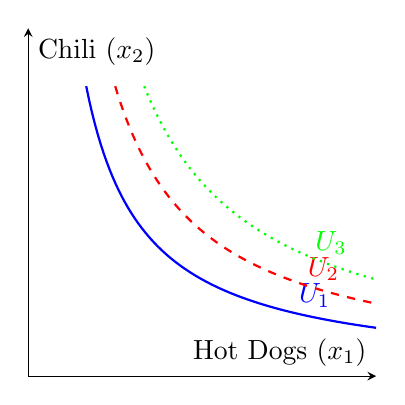
\begin{tikzpicture}
\begin{axis}[
    axis lines=middle,
    xmin=0, xmax=6,
    ymin=0, ymax=6,
    width=6cm, height=6cm,
    xlabel={Hot Dogs ($x_1$)},
    ylabel={Chili ($x_2$)},
    xtick=\empty, ytick=\empty
]

% Indifference Curves (Convex and downward sloping)
\addplot[thick, blue, domain=1:6, samples=100]
  ({x},{5/x})
  node[pos=0.85, above, blue] {$U_{1}$};

\addplot[thick, red, domain=1.5:6, samples=100, dashed]
  ({x},{7.5/x})
  node[pos=0.85, above, red] {$U_{2}$};

\addplot[thick, green, domain=2:6, samples=100, dotted]
  ({x},{10/x})
  node[pos=0.85, above, green] {$U_{3}$};

\end{axis}
\end{tikzpicture}
\caption{Indifference Curves for Hot Dogs and Chili (Both Preferred).}
\end{subfigure}
\hfill
%-----------------------------
% (b) Nuts (neutral) vs. Ice cream (liked)
%-----------------------------
\begin{subfigure}{0.32\textwidth}
\centering
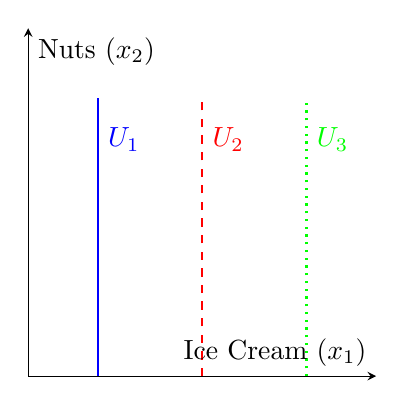
\begin{tikzpicture}
\begin{axis}[
    axis lines=middle,
    xmin=0, xmax=10,
    ymin=0, ymax=10,
    width=6cm, height=6cm,
    xlabel={Ice Cream ($x_1$)},
    ylabel={Nuts ($x_2$)},
    xtick=\empty, ytick=\empty
]

% Vertical Indifference Curves (Utility depends only on Ice Cream)
\addplot[thick, blue] coordinates {(2,0) (2,8)}
  node[pos=0.85, right, blue] {$U_{1}$};

\addplot[thick, red, dashed] coordinates {(5,0) (5,8)}
  node[pos=0.85, right, red] {$U_{2}$};

\addplot[thick, green, dotted] coordinates {(8,0) (8,8)}
  node[pos=0.85, right, green] {$U_{3}$};

\end{axis}
\end{tikzpicture}
\caption{Indifference Curves for Nuts (Neutral) and Ice Cream (Preferred).}
\end{subfigure}
\hfill
%-----------------------------
% (c) Orange (liked) vs. Broccoli (disliked)
%-----------------------------
\begin{subfigure}{0.32\textwidth}
\centering
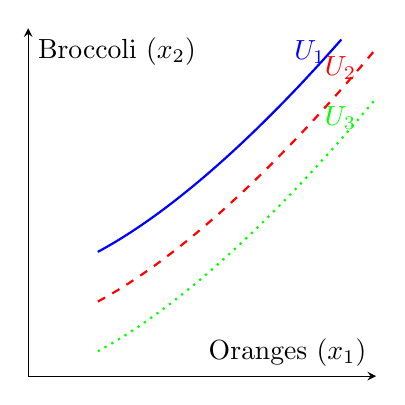
\begin{tikzpicture}
\begin{axis}[
    axis lines=middle,
    xmin=0, xmax=5,
    ymin=0, ymax=7,
    width=6cm, height=6cm,
    xlabel={Oranges ($x_1$)},
    ylabel={Broccoli ($x_2$)},
    xtick=\empty, ytick=\empty
]

% Indifference Curves (Convex and sloping downward)
\addplot[thick, blue, domain=1:4.5, samples=100]
  ({x},{0.5*x^1.5+2})
  node[pos=0.85, above, blue] {$U_1$};

\addplot[thick, red, dashed, domain=1:5, samples=100]
  ({x},{0.5*x^1.5 + 1})
  node[pos=0.85, above, red] {$U_2$};

\addplot[thick, green, dotted, domain=1:5, samples=100]
  ({x},{0.5*x^1.5})
  node[pos=0.85, above, green] {$U_3$};

\end{axis}
\end{tikzpicture}
\caption{Indifference Curves for Oranges (Preferred) and Broccoli (Disliked).}
\end{subfigure}

\caption{$u_{1} < U_{2} < U_{3}$}
\end{figure}

\vspace{1em}
\noindent
\textbf{Rubric for Question 1 (5 points):}
\begin{itemize}[noitemsep]
    \item[(+2pts)] Correct shape for two normal goods (downward-sloping).
    \item[(+2pts)] Correct depiction for a neutral good (vertical or horizontal IC).
    \item[(+1pt)] Correct depiction for a disliked good (upward-sloping IC).
\end{itemize}

\noindent\textbf{2.} Jennifer has \$10 to spend on tomatoes and cheese. The price of a pound of tomatoes is \$2 and the price of a pound of cheese is \$4. She has found her utility-maximizing bundle at 2 pounds of tomatoes and 1.5 pounds of cheese. Suppose Jennifer's income falls to \$8 and the price of tomatoes falls to \$1. The price of cheese remains the same. Jennifer is considering a bundle of zero units of tomatoes and 2 units of cheese. What is your advice? (5 points)
\noindent
\\\\\textbf{Advice:}\\
\begin{itemize}[noitemsep]
\vspace{-15pt}
\item With the new price of tomatoes (\$1) and the unchanged price of cheese (\$4), tomatoes are now relatively cheaper.
\item The bundle (0,2) spends all her \$8 on cheese alone. However, it was already affordable under the original budget and price scheme. Additionally, her previous optimal bundle (2,1.5) remains within her new budget. Since (0,2) was not optimal before and (2, 1.5)is still feasible now, (0,2) is unlikely to be the best choice. She should reconsider her marginal utility and find a new optimal bundle.
\end{itemize}
\textbf{Conclusion:} Buying zero tomatoes is \emph{not} optimal. She should \emph{re-optimize} with the new prices and reduced income.

\vspace{1em}
\noindent
\textbf{Rubric for Question 2 (5 points):}
\begin{itemize}[noitemsep]
    \item[(+3pts)] Reasoning
    \item[(+2pts)] True or False about whether (0,2) is optimal
\end{itemize}

\hrulefill

\section*{Part B: Long Questions (40 points)}

\textbf{1.} Consider a consumer who consumes only two goods, X and Y. His utility function for X and Y is given by $U(X,Y)= ln (X) + Y$, where ln represents the natural logarithm. 
\\a) Derive the consumer’s MRS of X for Y, using calculus to calculate his marginal utility from X and his marginal utility from Y. 
\\b) If the price of X is \$2, and the price of Y is \$4, and the consumer’s income spent on the two goods is \$100, What is the equation of Josh’s budget line? 
\\c) What are the optimal consumption choices, $X^*$ and $Y^*$ for this consumer? Show your work. (10 points)

\begin{enumerate}[label=(\alph*)]
    \item \textbf{Marginal Utilities and MRS} \\
    The consumer's utility function is
    \[
    U(X,Y) \;=\;\ln(X)\;+\;Y.
    \]
    \[
    \text{MU}_X \;=\;\frac{\partial U}{\partial X}\;=\;\frac{1}{X}, 
    \quad
    \text{MU}_Y \;=\;\frac{\partial U}{\partial Y}\;=\;1.
    \]
    The \textbf{marginal rate of substitution} of $X$ for $Y$ is
    \[
    \text{MRS}_{X,Y} = \frac{\text{MU}_X}{\text{MU}_Y} = \frac{\tfrac{1}{X}}{1} = \frac{1}{X}.
    \]

    \item \textbf{Budget Line} \\
    Prices are $P_X=2$ and $P_Y=4$, with income $M=100$. The budget constraint is
    \[
    2X \;+\;4Y \;=\;100.
    \]
    Or equivalently,
    \[
    Y \;=\;\frac{100 - 2X}{4} \;=\;25 \;-\;\tfrac{1}{2}X.
    \]

    \item \textbf{Optimal Consumption Choices \boldmath{$(X^*, Y^*)$}}\\
    The consumer maximizes utility where $\text{MRS}=\frac{P_X}{P_Y}$. That is,
    \[
    \frac{1}{X^*} \;=\;\frac{2}{4}\;=\;\tfrac12.
    \]
    Hence $X^* = 2$. Substituting $X^*=2$ into the budget line:
    \[
    2(2) + 4Y^* = 100
    \quad\Longrightarrow\quad
    4 \;+\;4Y^*\;=\;100
    \quad\Longrightarrow\quad
    Y^*=24.
    \]
    So the optimal bundle is
    \[
    (X^*, Y^*) = (2,\,24).
    \]
\end{enumerate}

\vspace{1em}
\noindent
\textbf{Rubric (10 points):}
\begin{itemize}[noitemsep]
    \item[(+3)] Correct marginal utilities(1pt for each) and MRS(1pt).
    \item[(+3)] Correct budget line equation.
    \item[(+4)] Correct solution for $X^*$ and $Y^*$(2pt for equation, 2pt for correct answer).
\end{itemize}

\noindent \textbf{2. } A consumer has $U= x^{0.5} y^{0.5}$ utility function where x and y are two goods. (15 points)
\begin{itemize}
    \item Find this consumer’s demands for goods x and y as functions of the prices and her income I.
\item Suppose that the price of good x is \$5, and the price of Y is \$10, Find out the optimal bundle of X and Y for this consumer. (when Income =50)
\item Suppose that the price of good 1 increase to \$10. What bundle of x and y does the consumer demand now?
\end{itemize}
\begin{enumerate}[label=(\roman*)]
    \item \textbf{Derive the Demand Functions} \\
    The utility is $U(x,y)=\sqrt{xy}$. Equivalently $U(x,y)=x^{1/2}y^{1/2}$. Prices are $p_x, p_y$, and income is $I$. \\
    The consumer maximizes
    \[
    x^{1/2}\,y^{1/2}
    \quad \text{subject to}
    \quad p_x\,x\;+\;p_y\,y \;=\;I.
    \]
    \[
 \text{MRS} = \frac{p_x}{p_y}
    \]
       \[
\text{Marginal utility of x} = \frac{1}{2}x^{-\frac{1}{2}}y^{\frac{1}{2}} \\
\text{Marginal utility of y} = \frac{1}{2}x^{\frac{1}{2}}y^{-\frac{1}{2}}
    \]
hence \[\text{MRS} = \frac{y}{x} = \frac{p_x}{p_y}\]
plug into the budget line: $p_{x} x + p_{y} y = I$ and we get
    \[
    x^* = \frac{I}{2\,p_x}, 
    \quad
    y^* = \frac{I}{2\,p_y}.
    \]

    \item \textbf{Optimal Bundle for $p_x=5, p_y=10, I=50$} \\
    Using $x^*=\tfrac{I}{2p_x}$ and $y^*=\tfrac{I}{2p_y}$:
    \[
    x^* = \frac{50}{2\times5} = \frac{50}{10} = 5,
    \quad
    y^* = \frac{50}{2\times10} = \frac{50}{20} = 2.5.
    \]
    So the consumer buys $(x^*, y^*)=(5,2.5).$

    \item \textbf{New Price of $x=10$. Find the Demands} \\
    Now $p_x=10, p_y=10, I=50.$ Again from $x^*=\tfrac{I}{2p_x}, y^*=\tfrac{I}{2p_y}$:
    \[
    x^* = \frac{50}{2\times10} = \frac{50}{20} = 2.5,
    \quad
    y^* = \frac{50}{2\times10} = 2.5.
    \]
    So the consumer buys $(x^*, y^*)=(2.5, 2.5).$

\end{enumerate}

\vspace{1em}
\noindent
\textbf{Rubric(15 points):}
\begin{itemize}[noitemsep]
    \item[(+5)] (2pt) Marginal utilities and MRS, (1pt) MRS = Price Ratio (2pt)Correct derivation of the demand functions as $x^*=\dfrac{I}{2p_x}, y^*=\dfrac{I}{2p_y}$. (Full pnts if they aruge x and y as symmetric?) 
    \item[(+5)] Correct plug-in for $p_x=5, p_y=10, I=50$.
    \item[(+5)] Correct bundle for new $p_x=10$ (and the same $p_y=10, I=50$).
\end{itemize}

\noindent \textbf{3.} 
Draw the substitution effect and an income effect for a normal good. (5 points)\\
\textbf{Rubric(5 points):}\\
(+3pts) Graph\\
(+2pts) Reasoning\\\\
When the price of a \emph{normal} good rises, the total quantity demanded decreases. Decompose this change into:
    \begin{itemize}[noitemsep]
        \item \emph{Substitution effect:} Move along the indifference curve to a point where the slope matches the new price ratio.
        \item \emph{Income effect:} Once the consumer is on the new price ratio, reduce (or increase) their ``purchasing power'' to the new budget line, shifting them to the final optimum. For a normal good, the income effect \emph{reinforces} the substitution effect.
    \end{itemize}
\begin{figure}[!ht]
\centering
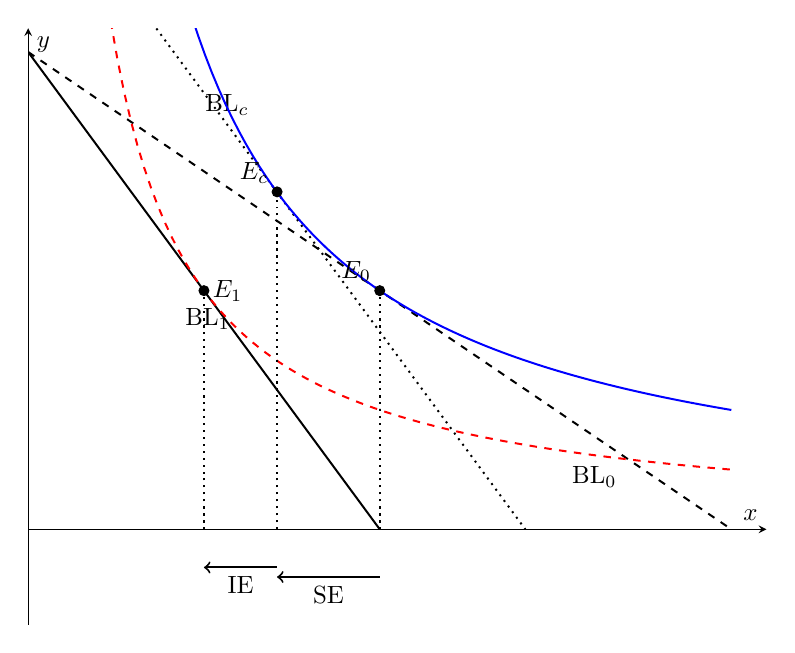
\begin{tikzpicture}[scale=0.9]

% Axis
\begin{axis}[
    axis lines=middle,
    xlabel={$x$},
    ylabel={$y$},
    xmin=0, xmax=10.5,
    ymin=-2, ymax=10.5,
    xtick = \empty,
    ytick = \empty,
    width=12cm, height=10cm,
    domain=0.1:10,
    samples=100
]
% 1) BL0: x+y=10
\addplot[thick, black, dashed, domain=0:10] 
    ({x},{10 - x})
    node[pos=0.85, below left] {BL$_0$};

% 2) BL1: 2x+y=10
\addplot[thick, black, domain=0:5] 
    ({x},{10 - 2*x})
    node[pos=0.6, above left] {BL$_1$};

% 3) BLc: y=14.14-2x
\addplot[thick, black, dotted, domain=0:7.07]
    ({x},{14.14 - 2*x})
    node[pos=0.4, above] {BL$_c$};

% 4) Indifference Curves
\addplot[thick, blue, domain=0.5:10] 
    ({x},{25/x});

\addplot[thick, red, dashed, domain=0.5:10]
    ({x},{12.5/x});

% 5) Mark Points E0=(5,5), E1=(2.5,5), E_c=(3.54,7.07)
\addplot[mark=*] coordinates {(5,5)};
\node[above left] at (axis cs:5,5) {$E_0$};

\addplot[mark=*] coordinates {(2.5,5)};
\node[right] at (axis cs:2.5,5) {$E_1$};

\addplot[mark=*] coordinates {(3.54,7.07)};
\node[above left] at (axis cs:3.54,7.07) {$E_c$};

% Vertical Lines at x=2.5, x=3.54, x=5
\addplot[thick, black, dotted, domain=0:5]
  ({2.5},{x});
\addplot[thick, black, dotted, domain=0:5]
  ({5},{x});
\addplot[thick, black, dotted, domain=0:7.07]
  ({3.54},{x});

\draw[<-, thick] 
  (axis cs:2.5, -0.8)  
  -- (axis cs:3.54, -0.8) 
  node[midway, below]{IE};  

\draw[<-, thick] 
  (axis cs:3.54, -1)  
  -- (axis cs:5, -1)  
  node[midway, below]{SE}; 
\end{axis}


\end{tikzpicture}
\caption{Substitution effect and Income effect for a normal good}
\label{fig:cobb-douglas-subs-income}
\end{figure}

\noindent \textbf{4.} Draw the substitution effect and income effect for an inferior good when there is an increase in price (10 points)\\
\textbf{Rubric(10 points):}\\
(6 pts) Graph\\
(4 pts) Reasoning\\\\
If the price of an \emph{inferior} good increases, the 
\emph{substitution effect} is the same direction---consume less of the good whose price rose. But the \emph{income effect} moves in the \emph{opposite} direction for an inferior good (the consumer's effective income shrinks, which might lead them to buy \emph{more} of that good if it is strongly inferior).

\begin{figure}[ht]
\centering
\begin{tikzpicture}
\begin{axis}[
    axis lines=middle,
    xmin=0, xmax=12,  % Extend x range
    ymin=-3, ymax=15,  % Extend y range
    width=12cm, height=8cm,
    xlabel={$x$}, ylabel={$y$},
    xtick=\empty, ytick=\empty
]

% -----------------------------------------------------------------
% 1) Budget Lines: BL_0 (initial), BL_1 (new), BL_c (compensated)
% -----------------------------------------------------------------
% BL_0 (old budget line)
\addplot[thick, black, domain=0:10]
  ({x},{10 - x})
  node[pos=0.8, above] {BL$_0$};

% BL_1 (new budget line: steeper slope due to px increase)
\addplot[thick, black, dashed, domain=0:5]
  ({x},{10 - 2*x})
  node[pos=0.8, below] {BL$_1$};

% BL_c (compensated budget line: same U as old but new px)
\addplot[thick, black, dotted, domain=0:6]
  ({x},{12 - 2*x})
  node[pos=0.4, above] {};

% -----------------------------------------------------------------
% 2) Indifference Curves: IC_0 (original), IC_1 (new)
% -----------------------------------------------------------------
\addplot[thick, blue, domain=4:6]
  ({x},{25/x})
  node[pos=0.85, above, blue] {};

\addplot[thick, red, domain=2:4, dashed]
  ({x},{18/x})
  node[pos=0.75, above, red] {};

\addplot[thick, green, domain=3:5, dashed]
  ({x},{128/x^3})
  node[pos=0.75, above, green] {};
% -----------------------------------------------------------------
% 3) Mark Optimal Points: E_0 (original), E_c (compensated), E_1 (final)
% -----------------------------------------------------------------
% E_0: Initial optimum
\addplot[mark=*] coordinates {(5,5)};
\node[above left] at (axis cs:5,5) {$E_0$};

% E_c: Compensated optimum (after sub effect)
\addplot[mark=*] coordinates {(3,6)};
\node[above right] at (axis cs:3,6) {$E_c$};

% E_1: Final optimum (after income effect)
\addplot[mark=*] coordinates {(4,2)};
\node[right] at (axis cs:4,2) {$E_1$};

% Vertical Lines at x=2.5, x=3.54, x=5
\addplot[thick, black, dotted, domain=0:5]
  ({5},{x});
\addplot[thick, black, dotted, domain=0:6]
  ({3},{x});
\addplot[thick, black, dotted, domain=0:2]
  ({4},{x});

\draw[->, thick] 
  (axis cs:5, -0.3)  
  -- (axis cs:3, -0.3) 
  node[midway, below]{SE};  

\draw[->, thick] 
  (axis cs:3, -1.2)  
  -- (axis cs:4, -1.2)  
  node[midway, below]{IE}; 
  
\end{axis}
\end{tikzpicture}
\caption{Substitution \& Income Effects for an Inferior Good ($x$ is Inferior)}
\end{figure}

\end{document}
